\section{Background and Related Work}
\subsection{Neighbor Sampling for GNNs}
One shortcoming of early GNN models is the large memory footprint.
As inspired by the Laplacian filter, they usually involve an adjacency matrix in each of their hidden layers, which scales up as the size of the graph increases.




To mitigate this, GraphSAGE~\cite{hamilton2017inductive} proposes neighbor sampling along with mini-batch.
It takes in the node pairs chosen in the mini-batch, their sampled neighbors, and multi-hop neighbors rather than the nodes in the whole graph.
This dramatically reduces the memory footprint.
A GraphSAGE model includes two to three aggregation layers, which can be mean, pooling, LSTM, etc.
Figure~\ref{fig:GrpahSAGE} shows an example of neighbor sampling on node 9.
Node indices are represented in hexadecimal.
Neighbors of node 9 are sampled, constituting the input of the second aggregation layer.
Similarly, the neighbors of these neighbors are sampled as the input for the first aggregation layer.
The input of the first aggregation layer is node features from the graph.
Consequently, the sampled node features are scattered in the node features tensor, as the illustration on the left shows.
Gathering needs to be done before DMA block transfer in the original mini-batch input transfer scheme, as Figure~\ref{fig:design_comparison}(a) shows.



\begin{figure}[!htbp]
    \centering
    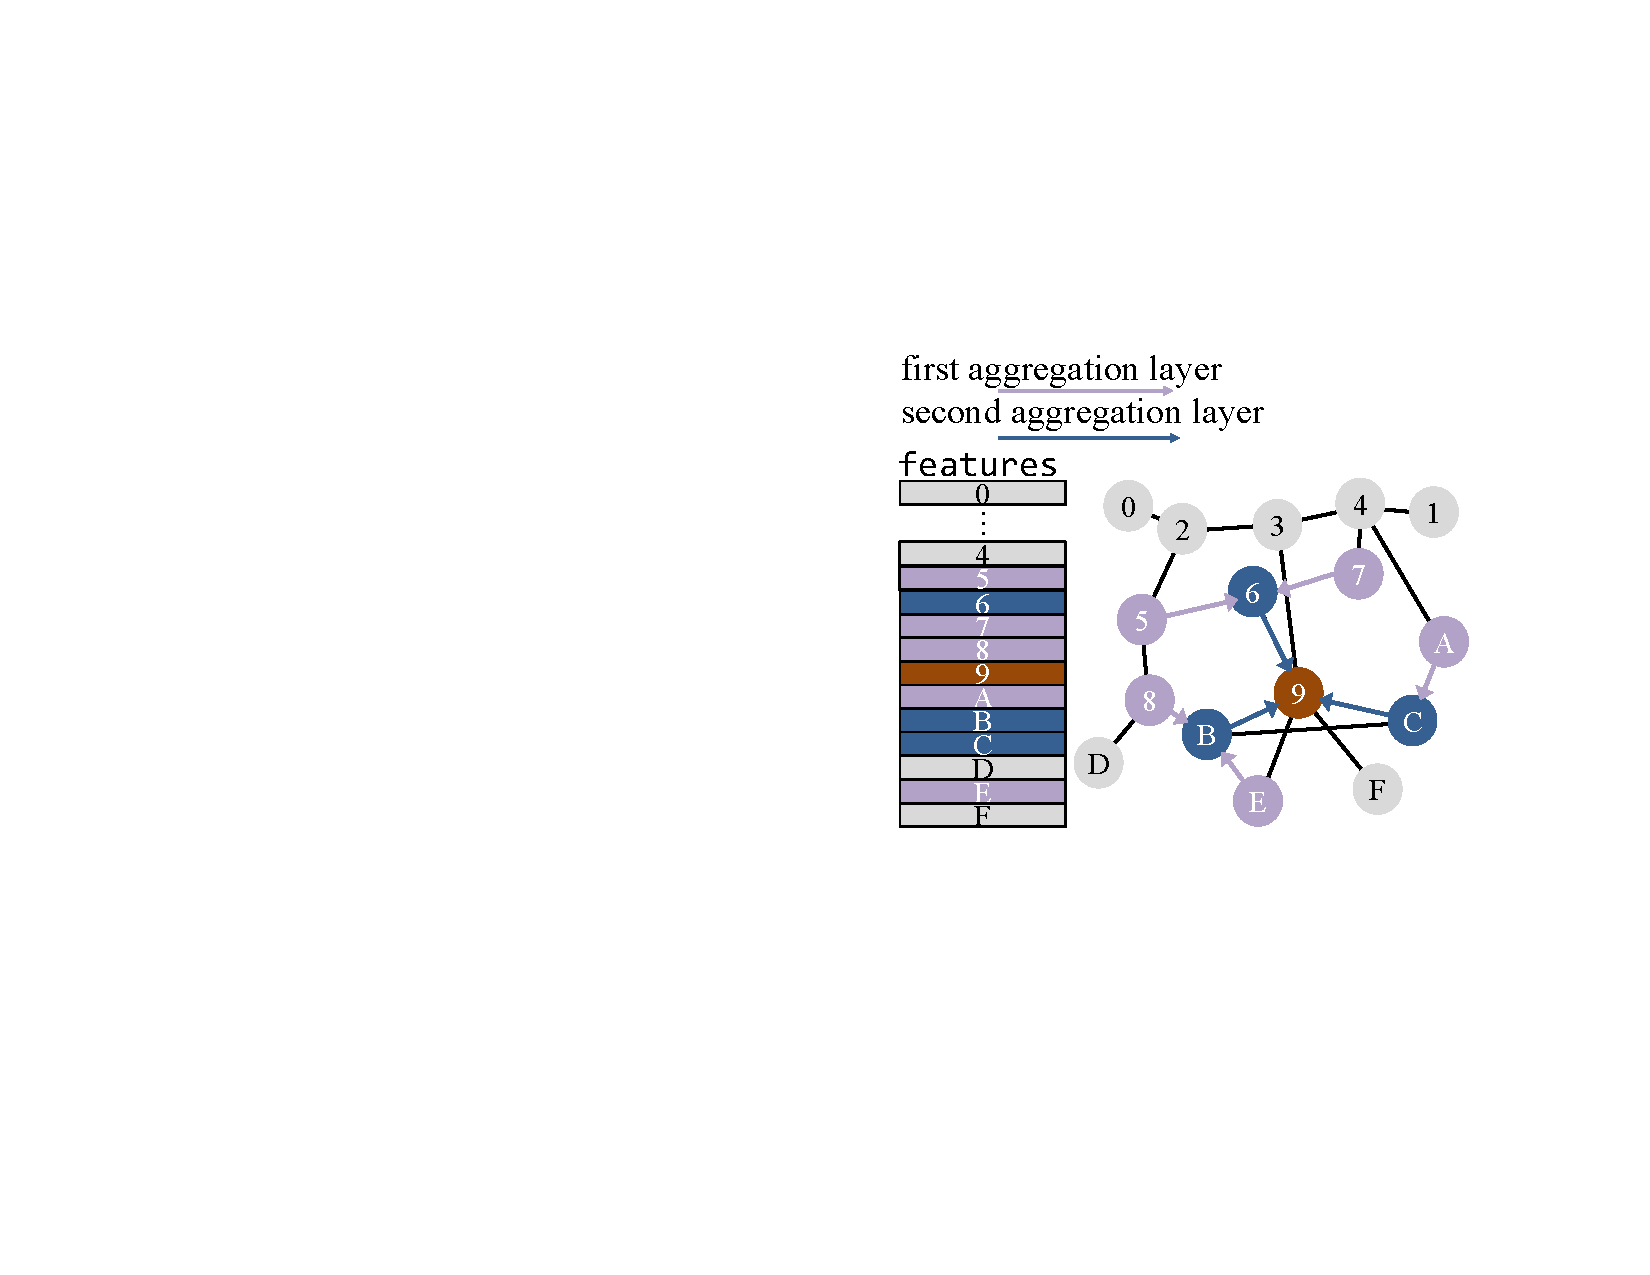
\includegraphics[width=0.5\linewidth]{figures/PyTorchDirect/GraphSAGE2_recolored.pdf}
    \caption{An example demonstrating the GraphSAGE neighbor sampling approach for output node 9. There are two aggregation layers in the model. The left shows the data layout of node features of this graph.}\label{fig:GrpahSAGE}
\end{figure}

\subsection{GPU Out-Of-Memory Solution for GNN Training}
In GNN training, the input features are located in a two-dimensional array where the row indices are the \kwc{identifiers} of nodes and the columns are the features of each node.
In Figure~\ref{fig:design_comparison}, we show a case of retrieving the node features of the neighboring nodes during the GNN training.
Due to the structural discrepancy between the graph and the array, accessing the features of neighboring nodes in the graph results in accessing rather unpredictable and non-sequential rows of the Feature Array.


A straightforward approach to sending these non-consecutive rows to the GPU is to call data copying functions like \texttt{cudaMemcpy()} multiple times, once for each row. 
Unfortunately, making multiple calls to data copying functions incurs significant overhead and can be highly inefficient. 
When the input graphs are small, one can bypass this issue by simply placing
the entire feature array into the GPU memory at the beginning of GNN training.
However, in reality, it is not reasonable to assume that the entire feature array can always fit into the GPU memory.

Currently, the solutions for training GNNs on huge graphs can be divided mainly into two categories:
1) Only the immediately necessary features for the current mini-batch are gathered by the CPU and then sent to the GPU memory~\cite{Pinterest}.
2) Before training, partition the input graphs into multiple smaller subgraphs that can be fit into the GPU memory and then train on them one by one~\cite{Chiang2019ClusterGCNAE,graphsaint-iclr20}.
In the former category, the CPU can become a bottleneck, slowing down the training pipeline. In the latter category, the subgraphs inevitably lose some of the distinct structural patterns of the original graphs~\cite{zu2019survey}.
PyTorch-Direct addresses these deficiencies by enabling the GPU to directly gather all the needed features from the host memory on demand.


\subsection{GNN Frameworks with Python DNN Libraries}
\kwc{To facilitate GNN development, efforts are made to create frameworks that incorporate commonly required functionalities in GNN training based on popular Python-based DNN libraries such as PyTorch and TensorFlow.}
DGL~\cite{wang2019deep} is developed based on MXNet, PyTorch, and TensorFlow. 
PyTorch-Geometric~\cite{fey2019fast} is a PyTorch-based GNN framework.
StellarGraph~\cite{StellarGraph} and Spektral~\cite{grattarola2020graph} are based on TensorFlow and Keras API. In PyTorch-Direct, we demonstrate the benefit of our approach by extending PyTorch.

\subsection{Large Scale GNN Systems}
There is rich literature \kwc{addressing the challenges of} large-scale GNNs.
While \kwc{this body of work highlights} the demands and issues with large-scale GNNs, the novelty of PyTorch-Direct is unique: it mitigates the PCIe bottleneck for these applications by proving the close-to-peak effective PCIe bandwidth of zero-copy in node features gathering and transfer and devising the new APIs and runtime modifications to integrate into PyTorch.
Works~\cite{sign_icml_grl2020,graphsaint-ipdps19,graphsaint-iclr20,Chiang2019ClusterGCNAE, Jia2020ImprovingTA} propose new models to mitigate the memory footprint, such as graph partitioning, layer sampling, etc. They change the algorithm and empirically may worsen the accuracy~\cite{ogbLeaderboard}.
In comparison, PyTorch-Direct applies to all GNN models using neighbor sampling.
Work~\cite{SAGA} proposes a general GNN processing framework able to utilize multiple GPUs and conduct high-level optimizations, including kernel fusions and dataflow optimizations. Still, it does not account for the PCIe transfer efficiency.
Work~\cite{zhengDistDGLDistributedGraph2020} devises a distributed CPU-only GNN processing system, which does not exploit the massive parallelism of GPU\kwc{s}.


Besides, there is much research on large-scale graph processing systems.
Work~\cite{10.14778/3384345.3384358} utilizes unified memory and static graph ordering to mitigate irregular data access, but our work \kwc{also} applies to dynamic graphs. Work~\cite{10.1145/3342195.3387537} proposes a subgraph generation algorithm and uses DMA engine\kwc{s} to perform host-to-device transfer.




\subsection{Ways of Data Transfer among CPU and GPUs}
There are three ways to transfer data among the CPU and GPUs, i.e., API calls for DMA transfers, on-demand paging by Unified Virtual Memory (UVM)~\cite{P100Whitepaper, V100Whitepaper, A100Whitepaper, UVMPrimer, pearson19}, and zero-copy access~\cite{UVMPrimer, minEMOGIEfficientMemoryaccess2020,relTransfer1}.

\kwc{The first way is through} explicit API calls.
Host logic in the program invokes the corresponding APIs to perform data transfer.
The two most commonly used APIs are \texttt{cudaMemcpy()} and \texttt{cudaMemcpyAsync()}, which perform synchronous and asynchronous data copy, respectively.
The programmer must also specify data movement direction, e.g., host to device, device to device, etc.
When the API is invoked, the driver uses the DMA engine to perform the transfer.
If the source data are in the host memory, \kwc{they} will be first copied to a pinned region in the host memory by the CPU, causing extra data movement~\cite{pearson19, gpudirectrdma}.
As Pearson et al.~\cite{pearson19}\ measured, the effective bandwidth is very low when the transfer size is a few KBs and reaches 50\% of the peak bandwidth only when the transfer size is at least 2\textsuperscript{17} to 2\textsuperscript{19} bytes.
Given that each node feature typically takes around 1 KB, the host must first gather the node features into a temporary array in host memory before DMA transfer to well utilize PCIe bandwidth.

On-demand paging is the second way. CUDA provides UVM~\cite{UVMPrimer} to reduce the burden of memory management.
\texttt{cudaMallocManaged()} \kwc{calls} allocate UVM-managed memory regions, which can be accessed by either the host or GPUs in the system.
During a miss, the driver transparently migrates the page from the remote to the local memory.
The migration granularity is between 4 KB and 2 MB.
\kwc{Since} Pascal architecture\kwc{, Nvidia GPUs use the page faulting mechanism to handle missing pages} when access\kwc{ing} a location not in its device memory~\cite{UVMPrimer2, P100Whitepaper}.
UVM provides the programmers with convenience.
Especially, they do not need to explicitly perform deep copies for every referenced memory region.
But \kwc{UVM} is not designed to maximize performance.
As Chien et al.~\cite{Chien_2019} have measured, page faults by unified virtual memory cause non-negligible negative impacts on bandwidth.
Besides, in GNN, in particular, only a few node features may be accessed per page migration, reducing the effective bandwidth.
Furthermore, since the \kwc{total} size of all node features is way larger than the device memory, it may cause excessive eviction, further aggravating the originally severe PCIe bottleneck.

The third method is zero-copy access.
GPU can access any data in the system as long as it is pinned and memory-mapped into the GPU's address space.
In zero-copy access, GPU sends the request through the interconnect to get data, without explicit copying or migration in the previously mentioned two mechanisms.
When accessing host memory, the GPU issues at most cacheline-sized, i.e., 128 bytes, data requests onto PCIe~\cite{minEMOGIEfficientMemoryaccess2020}.
There are three APIs or combinations that enable zero-copy in a memory region~\cite{min2021pytorchdirect}, but for simplicity, we choose \texttt{cudaMallocHost()} in PyTorch-Direct.


